\documentclass[sigconf,9pt]{acmart}

\usepackage{booktabs} % For formal tables
\usepackage{amsmath}
\usepackage{amsfonts}
\usepackage{microtype}
\usepackage{array}
\usepackage{multirow}
\usepackage{tabularx}
\usepackage{url}
\usepackage{tikz}
\usetikzlibrary{shapes.geometric, arrows, positioning, fit, backgrounds}

% Disable ACM copyright/permission block for submission
\settopmatter{printacmref=false}
\setcopyright{none}
\renewcommand\footnotetextcopyrightpermission[1]{}
\pagestyle{plain}

\acmConference[Middleware '26 Industry Track]{27th ACM International Middleware Conference}{December 14--18, 2026}{Tarragona, Spain}
\acmYear{2026}
\acmDOI{}
\acmISBN{}

% Compact padding
\setlength{\tabcolsep}{3pt}

% Compact bibliography spacing
\let\oldthebibliography\thebibliography
\let\endoldthebibliography\endthebibliography
\renewenvironment{thebibliography}[1]{%
  \begin{oldthebibliography}{#1}%
    \setlength{\itemsep}{0.5pt}%
    \setlength{\parskip}{0pt}%
  \small
}{%
  \end{oldthebibliography}%
}

\begin{document}

\title[Middleware-Centric Architectural Digital Model for Naval CMS]{A Middleware-Centric Architectural Digital Model for Pre-Deployment Verification and CI/CD Gating in Naval Combat Management Systems (Industry Track)}

\author{Ibrahim Onuralp Yigit}
\affiliation{%
  \institution{Command Control and Defense Technologies, HAVELSAN}
  \city{Istanbul}
  \country{Turkiye}
}
\email{iyigit@havelsan.com.tr}

\author{Onurcan Ersen}
\affiliation{%
  \institution{Command Control and Defense Technologies, HAVELSAN}
  \city{Istanbul}
  \country{Turkiye}
}
\email{oersen@havelsan.com.tr}

\author{Mustafa Can Caliskan}
\affiliation{%
  \institution{Command Control and Defense Technologies, HAVELSAN}
  \city{Istanbul}
  \country{Turkiye}
}
\email{mcaliskan@havelsan.com.tr}

\begin{abstract}
Modern mission-critical Naval Combat Management Systems (CMS), such as HAVELSAN's combat-proven ADVENT CMS, are distributed real-time systems built on publish/subscribe middleware, integrating hundreds of applications across operator consoles, radar trackers, weapon controllers, and tactical data links. Their most severe integration defects are non-local architectural misconfigurations: incompatible Quality-of-Service (QoS) contracts on hard-deadline weapon assignment channels, overlapping CPU core affinity masks, orphaned tactical topics, and circular package dependencies. Such defects survive unit and component testing and surface only during shipyard integration or sea trials.

We report on \emph{System as a Graph} (SaaG), an architectural digital model for pre-deployment verification and CI/CD gating. Reconstructed from candidate release descriptors rather than runtime synchronization, SaaG builds an attributed typed multigraph ($G = (V, E, \tau_V, \tau_E, w_V, w_E)$) over applications, brokers, topics, processing nodes, and shared libraries; derives asymmetric failure-dependency projections from pub/sub topology ($B \xrightarrow{\text{DEPENDS\_ON}} A$); and gates the pipeline on static rule violations ranked by a severity rubric adapted from MIL-STD-882E.

Our central industrial finding is clear: graph analysis is not the computational bottleneck. Across five scaling operational naval platform profiles (1,498 to 3,254 components across up to 66 distributed nodes), static verification executes in 0.125\,s on a single-node airborne profile and 1.152\,s on the 66-node flagship profile (P95 1.161\,s), representing under 0.22\% of a typical 9-minute automated build pipeline. The rule catalog targets pub/sub misconfiguration classes that would otherwise surface only on physical testbeds. However, an industrial gap analysis reveals that of seven verification capabilities specified with naval combat system architects, six remain constrained by configuration-data acquisition across defense engineering silos rather than by algorithmic limits. We report the framework architecture, multi-scale verification latency, the misconfiguration classes the catalog targets, and practical lessons from building the prototype inside a defense engineering organization.
\end{abstract}

\begin{CCSXML}
<ccs2012>
   <concept>
       <concept_id>10010520.10010575.10010577</concept_id>
       <concept_desc>Computer systems organization~Reliability</concept_desc>
       <concept_significance>500</concept_significance>
   </concept>
   <concept>
       <concept_id>10011007.10011074.10011099.10011102</concept_id>
       <concept_desc>Software and its engineering~Software defect analysis</concept_desc>
       <concept_significance>500</concept_significance>
   </concept>
</ccs2012>
\end{CCSXML}

\ccsdesc[500]{Computer systems organization~Reliability}
\ccsdesc[500]{Software and its engineering~Software defect analysis}

\keywords{Naval Combat Management Systems (CMS), ADVENT CMS, SaaG Framework, Architectural Digital Model, Middleware Verification, Pub/Sub QoS Contracts, CI/CD Gating, CPU Core Pinning, Static Rule Auditing, OMG DDS, MIL-STD-882E, Network Enabled Capability (NEC)}

\maketitle

\section{Introduction \& Industrial Problem Statement}

Continuous Integration and Continuous Delivery (CI/CD) pipelines have fundamentally transformed software engineering by automating compilation, testing, and artifact generation~\cite{humble2010}. In naval defense systems, modern Combat Management Systems (CMS) have evolved from monolithic mainframes into modular, distributed, open-architecture systems governed by high-performance publish/subscribe (pub/sub) middleware~\cite{omg2015dds}.

\subsection{The Pre-Deployment Verification Gap in Naval Combat Systems}

Modern naval operations require rapid sensor-to-shooter loops, multi-sensor data fusion, coordinated weapon assignment, and seamless cross-platform interoperability. Built to fulfill these demands, \textbf{ADVENT CMS} (developed by \textbf{HAVELSAN} in cooperation with the Turkish Naval Forces Research Center Command---ARMERKOM~\cite{advent2022}) represents a state-of-the-art naval combat suite spanning a wide product tree: \textbf{ADVENT Kalyon} and \textbf{Milgem CMS} for surface combatants (frigates, corvettes, MCM vessels) handling multi-threat warfare (AAW, ASuW, ASW, EW); \textbf{LHD CMS} for amphibious assault flagships (e.g., L400 TCG Anadolu), providing task group command, multi-link gateway centers, and unmanned vehicle control; \textbf{ADVENT Rota}, a mission management system for USV/UUV/UAV platforms with STANAG 4586 compliance~\cite{stanag4586}; \textbf{ADVENT Mart\i}, an airborne C2 system for maritime patrol aircraft and naval helicopters; and \textbf{ADVENT Ufuk}, a land-based coastal surveillance and C2 system compiling the Recognized Maritime Picture.

Across these platforms, ADVENT CMS comprises over \textbf{155 external system integrations}, \textbf{750 distributed software applications}, and \textbf{13,000,000 lines of code}. Subsystems communicate over \textbf{Genieware}, a national publish/subscribe middleware for real-time mission-critical defense systems. Genieware adopts the OMG DDS~\cite{omg2015dds} data-centric model and its Request/Offered (RxO) contract semantics for the \texttt{RELIABILITY}, \texttt{DURABILITY}, \texttt{PARTITION}, and \texttt{DOMAIN\_ID} policies---precisely the policies our rules evaluate---so we use DDS terminology throughout and the rules of \S3 apply unchanged to DDS deployments. Genieware diverges in its discovery and wire protocol, which our static model does not represent. Platforms also interoperate over Tactical Data Links (TDLs: Link 11, Link 16~\cite{stanag5516}, Link 22~\cite{stanag5522}, and ADVENT Native Link H). Under the \textbf{Network Enabled Capability (NEC)} paradigm, ADVENT shares sensor tracks and weapon allocations across platforms, enabling Force-Wide Weapon/Sensor Allocation (WASA) and remote firing authorizations.

\begin{figure}[t]
\centering
\resizebox{\columnwidth}{!}{%
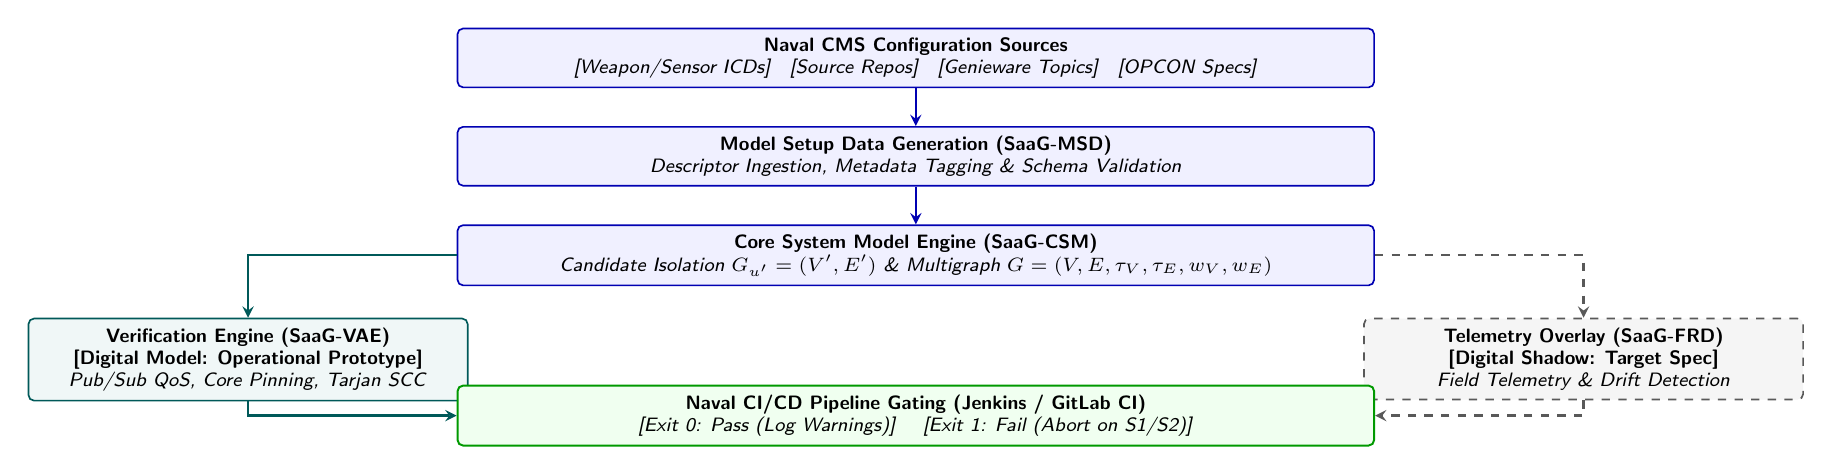
\begin{tikzpicture}[node distance=0.48cm, font=\sf\scriptsize, >=stealth]
  \tikzstyle{block} = [draw=blue!70!black, fill=blue!6, rectangle, rounded corners=2pt, minimum width=0.96\columnwidth, minimum height=0.42cm, align=center, line width=0.6pt]
  \tikzstyle{subblock} = [draw=teal!70!black, fill=teal!6, rectangle, rounded corners=2pt, minimum width=0.46\columnwidth, minimum height=0.50cm, align=center, line width=0.6pt]
  \tikzstyle{dashedblock} = [draw=gray!70!black, dashed, fill=gray!8, rectangle, rounded corners=2pt, minimum width=0.46\columnwidth, minimum height=0.50cm, align=center, line width=0.6pt]
  \tikzstyle{gateblock} = [draw=green!60!black, fill=green!6, rectangle, rounded corners=2pt, minimum width=0.96\columnwidth, minimum height=0.42cm, align=center, line width=0.7pt]

  \node (sources) [block] {\textbf{Naval CMS Configuration Sources}\\ \textit{[Weapon/Sensor ICDs] \; [Source Repos] \; [Genieware Topics] \; [OPCON Specs]}};
  \node (msd) [block, below=of sources] {\textbf{Model Setup Data Generation (SaaG-MSD)}\\ \textit{Descriptor Ingestion, Metadata Tagging \& Schema Validation}};
  \node (csm) [block, below=of msd] {\textbf{Core System Model Engine (SaaG-CSM)}\\ \textit{Candidate Isolation $G_{u'} = (V', E')$ \& Multigraph $G = (V, E, \tau_V, \tau_E, w_V, w_E)$}};
  
  \node (vae) [subblock, below left=0.40cm and -0.15cm of csm] {\textbf{Verification Engine (SaaG-VAE)}\\ \textbf{\scriptsize[Digital Model: Operational Prototype]}\\ \textit{Pub/Sub QoS, Core Pinning, Tarjan SCC}};
  \node (frd) [dashedblock, below right=0.40cm and -0.15cm of csm] {\textbf{Telemetry Overlay (SaaG-FRD)}\\ \textbf{\scriptsize[Digital Shadow: Target Spec]}\\ \textit{Field Telemetry \& Drift Detection}};
  
  \node (gate) [gateblock, below=1.25cm of csm] {\textbf{Naval CI/CD Pipeline Gating (Jenkins / GitLab CI)}\\ \textit{[Exit 0: Pass (Log Warnings)] \quad [Exit 1: Fail (Abort on S1/S2)]}};
  
  \draw[->, thick, blue!70!black] (sources) -- (msd);
  \draw[->, thick, blue!70!black] (msd) -- (csm);
  \draw[->, thick, teal!70!black] (csm) -| (vae);
  \draw[->, thick, dashed, gray!70!black] (csm) -| (frd);
  \draw[->, thick, teal!70!black] (vae) |- (gate);
  \draw[->, thick, dashed, gray!70!black] (frd) |- (gate);
\end{tikzpicture}%
}
\caption{SaaG pipeline integration for ADVENT CMS. Dashed boxes are specified, not yet built.}
\label{fig:architecture}
\end{figure}

When a candidate software build is submitted for release into an operational naval platform, conventional CI/CD pipelines evaluate unit and module tests in isolation, so non-local architectural misconfigurations slip through. Latency-critical track fusion daemons or fire control calculators are pinned to CPU core masks overlapping non-real-time GUI renderers or loggers on the same multi-core console. Endpoints are bound with incompatible Request/Offered (RxO) QoS contracts---a weapon assignment subscriber requesting \texttt{TRANSIENT\_LOCAL} durability against a fire control publisher offering only \texttt{VOLATILE}---so the endpoints never match and data never flows; the middleware raises an incompatible-QoS status, but operational code rarely traps it, making the failure effectively silent. Topic schemas diverge across platform releases, or refactored TDL forwarding topics are left with zero subscribers. And transitive dependency cycles between weapon allocation planners and threat evaluation modules surface as initialization deadlocks during OPCON start-up.

Provisioning full target hardware testbeds (physical multi-console Combat Information Centers [CIC], real sensor/weapon simulators, and multi-ship test ranges) for every candidate release is prohibitively expensive, logistically complex, and slow. Leaving architectural defects to be discovered during shipyard commissioning, harbor acceptance tests (HAT), or sea acceptance tests (SAT) leads to massive project delays and severe safety risks.

\subsection{The Architectural Digital Model Paradigm \& Dual Operational Usages}

To eliminate this pre-deployment gap and manage system complexity across the lifecycle, we developed \textbf{System as a Graph (SaaG)}. Rather than relying on heavyweight runtime testbeds, SaaG constructs an attributed graph model of the target combat system topology directly from configuration artifacts and interface contracts.

The digital twin classification of Kritzinger et al.~\cite{kritzinger2018} distinguishes a \textbf{digital model} (no automated exchange with the physical system; built from static artifacts), a \textbf{digital shadow} (automated one-way flow from the physical system to the model), and a \textbf{digital twin} (automated bidirectional synchronization). Under this taxonomy our framework is strictly an \emph{architectural digital model}---reconstructed deterministically from configuration artifacts. In naval engineering practice, the architectural digital model serves two complementary operational usages: (1) \textbf{Pre-Deployment Verification \& CI/CD Gating}, preventing non-conforming builds ($G_{u'}$) from reaching integration testbeds; and (2) \textbf{Architectural Improvement \& Refactoring of Existing Platforms}, enabling architects to detect circular dependency cycles, discover criticality bottlenecks, prune dead topic configurations, and perform ``what-if'' impact simulations across fielded combat systems.

\subsection{Key Industrial Contributions \& Empirical Findings}

This paper makes the following contributions:
\begin{enumerate}\itemsep=0.5pt
    \item \textbf{Naval CMS Architectural Model Baseline (\S2):} A formal directed multigraph representation ($G = (V, E, \tau_V, \tau_E, w_V, w_E)$) capturing 5 entity classes, 6 structural relations, and 6 failure-dependency projection rules that explicitly map the downstream propagation of architectural risk in pub/sub naval combat systems.
    \item \textbf{CI/CD Pipeline Gating \& Verification Methodology (\S3, \S4):} A two-stage deployment gate operating on standard CI runners with a defined safety severity rubric (S1--S4) adapted from MIL-STD-882E~\cite{milstd882e}. We characterize the mission-critical pub/sub misconfiguration classes the rule catalog targets (QoS mismatches, CPU core contention, topic continuity breaks, circular dependencies) and state which are covered by rules implemented in the prototype.
    \item \textbf{Verification Complexity \& Industrial Bottleneck Analysis (\S5, \S6):} Benchmarks across 5 naval platform profiles (1,498--3,254 components; 1--66 nodes) modeled on ADVENT platform lines show gate latency of 0.125--1.152\,s, under 0.22\% of a 9-minute build, with node distribution rather than component count driving cost. We document that 6 of 7 specified verification capabilities are blocked by configuration data acquisition across defense engineering silos, not by algorithmic complexity.
\end{enumerate}

\section{The Architectural Digital Model: Formulation and Graph Derivation}

SaaG adopts and operationalizes the formal graph modeling foundation established by Yigit and Buzluca~\cite{yigit2025graph} for distributed publish-subscribe systems. We formalize the distributed naval CMS middleware topology as an attributed, weighted directed multigraph:
\begin{equation}
G = (V, E, \tau_V, \tau_E, w_V, w_E)
\end{equation}

\subsection{Entity Classes and Structural Relations}

The vertex set $V$ is partitioned into five distinct entity types ($\tau_V: V \to \mathcal{T}_v$):
\begin{itemize}\itemsep=0.5pt
    \item \textbf{Applications ($V_{\text{app}}$):} Executable CMS software binaries.
    \item \textbf{Brokers ($V_{\text{broker}}$):} Broker services facilitating CMS communication.
    \item \textbf{Topics ($V_{\text{topic}}$):} Typed publish/subscribe communication channels carrying data payloads.
    \item \textbf{Infrastructure Nodes ($V_{\text{node}}$):} Physical OPCON console workstations, ruggedized VME/VPX server chassis, and mission computers.
    \item \textbf{Libraries ($V_{\text{lib}}$):} Shared dynamic libraries.
\end{itemize}

Six structural edge types ($\tau_E: E_{\text{structural}} \to \mathcal{T}_e$) are extracted directly from configuration descriptors: \texttt{PUBLISHES\_TO}, \texttt{SUBSCRIBES\_TO}, \texttt{ROUTES}, \texttt{RUNS\_ON}, \texttt{CONNECTS\_TO}, and \texttt{USES}. We additionally write \texttt{COLOCATED\_WITH} for the symmetric relation \emph{induced} by two units sharing a \texttt{RUNS\_ON} target; it is derived rather than ingested, and is used in Table~\ref{tab:dep_rules}.

\subsection{Asymmetric Failure-Dependency Projection}

In pub/sub middleware, data messages flow from publisher to subscriber ($A \to B$). However, \textbf{structural failure dependency points in the exact opposite direction ($B \xrightarrow{\text{DEPENDS\_ON}} A$)}: if Publisher $A$ (e.g., radar tracker) fails or produces corrupt messages, Subscriber $B$ (e.g., fire control calculator) is starved or degraded; conversely, if Subscriber $B$ crashes, Publisher $A$ continues unaffected.

Building upon the dependency analysis methodology of Yigit and Buzluca~\cite{yigit2025graph}, SaaG projects logical \texttt{DEPENDS\_ON} edges from structural topology (Table~\ref{tab:dep_rules}).

\begin{table}[h]
\centering
\caption{Derived Logical Dependency Edge Projection Rules.}
\label{tab:dep_rules}
\small
\begin{tabularx}{\columnwidth}{c l X c}
\toprule
\textbf{Rule} & \textbf{Type} & \textbf{Derivation Pattern} & \textbf{Weight $w(e)$} \\
\midrule
1 & \texttt{app\_to\_app} & App/Lib \texttt{SUB} $t \leftarrow$ \texttt{PUB} App/Lib & $\max_{t} w(t)$ \\
2 & \texttt{app\_to\_broker} & App/Lib \texttt{PUB}/\texttt{SUB} $t \leftarrow$ \texttt{ROUTES} Broker & $\max_{t} w(t)$ \\
3 & \texttt{node\_to\_node} & Lifted from \texttt{app\_to\_app} between hosted units & Lifted $\max(w)$ \\
4 & \texttt{node\_to\_broker} & Lifted from \texttt{app\_to\_broker} for hosted units & Lifted $\max(w)$ \\
5 & \texttt{app\_to\_lib} & App/Lib \texttt{USES} $\rightarrow$ Library & Inherits $w(\text{app})$ \\
6 & \texttt{broker\_to\_broker} & Colocation edge sharing physical Node & Inherits $w(\text{node})$ \\
\bottomrule
\end{tabularx}
\end{table}

\subsection{Intrinsic QoS \& Criticality Weight Propagation}

SaaG assigns criticality weights $w(v) \in [0, 1]$ across all entities via an expert-elicited linear weighting of QoS contracts, normalized message size, and topology fan-out:

\begin{enumerate}\itemsep=0.5pt
    \item \textbf{Intrinsic Topic Weight Formula:} For each topic $t \in V_{\text{topic}}$,
    \begin{equation}
    w(t) = \max\left(0.01, \; \beta \cdot \text{QoS\_score}(t) + (1 - \beta) \cdot \text{size\_norm}(t)\right)
    \end{equation}
    where $\beta = 0.85$, $\text{size\_norm}(t) = \min\left(\frac{\log_2(1 + \text{size\_kb})}{50}, \, 1.0\right)$, and:
    \begin{equation}
    \text{QoS\_score}(t) = 0.30 \cdot \text{rel} + 0.40 \cdot \text{dur} + 0.30 \cdot \text{prio}
    \end{equation}
    Reliability (\texttt{RELIABLE}=1.0, \texttt{BEST\_EFFORT}=0.0), Durability (\texttt{PERSISTENT}=1.0, \texttt{TRANSIENT\_LOCAL}=0.5, \texttt{VOLATILE}=0.0), and Transport Priority (\texttt{CRITICAL}=1.0, \texttt{HIGH}=0.66, \texttt{LOW}=0.0).

    \item \textbf{Upward Weight Propagation:} Applications and brokers inherit from the topics $T(x)$ they touch,
    \begin{equation}
    w(x) = \alpha_x \max_{t \in T(x)} w(t) + (1-\alpha_x)\operatorname{mean}_{t \in T(x)} w(t)
    \end{equation}
    with $\alpha_{\text{app}}=0.80$ and $\alpha_{\text{broker}}=0.70$. Libraries amplify with fan-out, $w(l) = \min(1.0,\, \text{base\_w}\,(1 + \gamma \log_2(1 + DG_{\text{in}}(l))))$ where $\text{base\_w}=0.20$, $\gamma=0.15$, and $DG_{\text{in}}(l)$ is the in-degree of $l$; a node takes the maximum of what it hosts, $w(n) = \max_{v\,\text{RUNS\_ON}\,n} w(v)$.
\end{enumerate}

\subsection{Operational Usages: Pipeline Gating and Platform Refactoring}

The architectural digital model serves two complementary functions across the naval combat system lifecycle:

\noindent\textbf{1. Pre-Deployment Verification \& Pipeline Gating (Forward Mode):} During concurrent CI/CD pipeline builds, SaaG instantiates an isolated candidate graph $G_{u'} = (V', E')$ by substituting candidate unit version $u'$ into the baseline platform inventory, guaranteeing baseline immutability. The runner audits $G_{u'}$ against static middleware rules (\S3) in $<1.2$\,s, enforcing fail-closed gating on safety-critical S1/S2 violations.

\noindent\textbf{2. Architectural Improvement \& Platform Refactoring (Diagnostic Mode):} Beyond release gating, architects query the global baseline model $G_{\text{baseline}}$ to drive systemic refactoring: Tarjan's SCC extracts cyclic subgraphs across legacy packages (e.g., WASA allocation against threat evaluation) for decoupling into layered abstractions; topology fan-out combined with intrinsic weights $w(v)$ pinpoints overloaded brokers and high-fanout topics needing replication or decomposition; orphaned topics ($|P(t)|=0$ or $|S(t)|=0$) and unreferenced libraries ($DG_{\text{in}}(l)=0$) expose accumulated configuration debt; and proposed structural changes---migrating applications across hosts, altering a durability contract---can be simulated on the model before production source is touched.

\section{Model-Driven Verification Rules \& CI/CD Pipeline Gating}

SaaG enforces static compliance rules over $G_{u'}$. Table~\ref{tab:rules} separates rules implemented in the prototype (SaaG-P, $\bullet$), which are audited statically on descriptors today, from those specified for the target enterprise integration but not yet realized ($\circ$).

\begin{table}[h]
\centering
\caption{Verification Rules Catalog ($\bullet$ Implemented; $\circ$ Specified).}
\label{tab:rules}
\small
\begin{tabularx}{\columnwidth}{l c c X}
\toprule
\textbf{Policy / Rule} & \textbf{SaaG-P} & \textbf{SaaG-D} & \textbf{Target Middleware Check} \\
\midrule
Pub/Sub RxO QoS Matching & $\bullet$ & $\bullet$ & Durability \& Reliability ($O \ge R$) \\
CPU Core Allocation & $\bullet$ & $\bullet$ & Core count $\le C(v_p)$ per host \\
CPU Core Non-Overlap & $\circ$ & $\bullet$ & Pairwise non-overlapping masks \\
Topic Continuity & $\bullet$ & $\bullet$ & Orphaned topics ($|P|=0 \lor |S|=0$) \\
Tactical Schema Match & $\bullet$ & $\bullet$ & TDL / Link 16 / STANAG match \\
Circular Dependencies & $\bullet$ & $\bullet$ & Tarjan's SCC on dependencies \\
Telemetry Drift & $\circ$ & $\bullet$ & $E_{\text{Observed}} \setminus E_{\text{Designed}}$ via logs \\
\bottomrule
\end{tabularx}
\end{table}

\subsection{Severity Rubric \& Alignment with Military Safety Standards (MIL-STD-882E)}

MIL-STD-882E~\cite{milstd882e} classifies the severity of \emph{mishap consequences}, not of static configuration defects, so we \emph{adapt} rather than adopt its four-level scale: each violation is assigned the severity of the worst credible mishap it could contribute to, given the criticality of the channels and hosts it affects. Severity is deliberately decoupled from message transport priority, since a \texttt{LOW}-priority channel may still gate a safety-critical function:
\begin{itemize}\itemsep=0.5pt
    \item \textbf{S1 (Critical Severity --- Catastrophic / Safety Critical):} Flaws causing complete loss of safety-critical functions (e.g., pub/sub RxO mismatch on weapon assignment or primary radar tracking channels, CPU over-allocation on fire control servers).
    \item \textbf{S2 (High Severity --- Critical / Mission Essential):} Severe defects with localized redundancy or secondary mitigation (e.g., orphaned tactical data link topics, circular dependencies among core WASA engagement planning units).
    \item \textbf{S3 (Medium Severity --- Marginal / Operational):} Non-critical configuration anomalies (e.g., unassigned transport priority hints, best-effort auxiliary sensor stream topic leaks).
    \item \textbf{S4 (Low Severity / Informational):} Style and maintenance warnings (e.g., deprecated utility library versions, non-standard topic naming).
\end{itemize}

\subsection{CI/CD Runner Integration: Exit Codes, Delta-Aware Gating, \& Waiver Register}

SaaG integrates into standard Jenkins and GitLab CI/CD runners via a CLI gate:
\begin{equation}
\text{Exit} = \begin{cases} 0, & \text{PASS: No S1/S2 violations (S3/S4 logged)} \\ 1, & \text{FAIL: S1 (Critical) or S2 (High) detected} \\ 2, & \text{ERROR: Execution / parse failure} \end{cases}
\end{equation}

Standard CI runners treat non-zero exit codes as build failures. On safety-critical release branches (weapon control, fire authorization, track fusion) SaaG runs \textbf{fail-closed}: a tool error (Exit 2) is treated as a gate failure and aborts the pipeline, so a candidate that cannot be analyzed is never allowed through unverified. Non-tactical auxiliary branches may run fail-open, logging Exit 2 as a warning with mandatory audit capture.

\subsubsection{Delta-Aware Gating \& Waiver Register}
In legacy naval codebases carrying pre-existing technical debt, an absolute gate blocks every build if baseline violations exist. SaaG supports \emph{delta-aware gating}: candidate builds are blocked only if $\text{Violations}(G_{u'}) \setminus \text{Violations}(G_{\text{baseline}}) \neq \emptyset$. Known legacy violations are managed via a Chief Architect-approved \emph{Waiver Register} with cryptographic signatures and expiration dates.

\section{Multi-Scale Naval Platform Architectures \& Verification Methodology}

To assess the practical applicability of SaaG pre-deployment verification in an operational naval combat systems environment, we model the architectural scales and middleware configurations across five major ADVENT platform families (\textbf{ADVENT Martı}, \textbf{ADVENT Ufuk}, \textbf{ADVENT Rota}, \textbf{ADVENT Kalyon / Milgem CMS}, and \textbf{LHD CMS Flagship}).

\subsection{Multi-Domain Combat System Architecture \& Platform Profiles}

Modern naval combat suites deploy across diverse physical and operational domains, as reflected in the public ADVENT product tree. \textbf{Martı} is an airborne C2 fit for maritime patrol aircraft, helicopters, and naval UAVs, handling airborne radar, sonobuoy acoustic processing, and data link relay in a tight single-node footprint ($|V|=1{,}498$, $|E|=4{,}824$). \textbf{Ufuk} is a land-based multi-sensor compilation center integrating coastal radar, AIS, ADS-B, and electro-optical surveillance across 23 server nodes ($|V|=2{,}174$, $|E|=7{,}142$). \textbf{Rota} is the mission management system for USV/UUV/UAV platforms with STANAG 4586 compliance~\cite{stanag4586} ($|V|=2{,}192$, $|E|=6{,}980$). \textbf{Milgem CMS / Kalyon} is the multi-warfare surface combatant suite (AAW, ASuW, ASW, EW) across 21 console nodes ($|V|=3{,}254$, $|E|=11{,}460$). \textbf{LHD CMS} is the task group flagship fit (e.g., L400 TCG Anadolu) with multi-link gateway centers and joint operations planning over 66 consoles and server chassis ($|V|=2{,}775$, $|E|=9{,}620$).

Across all platform scales, subsystems rely on \textbf{Genieware} publish/subscribe middleware to facilitate real-time sensor-to-shooter coordination and Network Enabled Capability (NEC).

\subsection{Continuous Verification \& Pipeline Gating Workflow}

On every merge request, SaaG runs inside the CI runner (Jenkins, GitLab CI) in four stages. It extracts candidate unit descriptors, IDL schemas, topic bindings, and node affinity masks and builds the isolated candidate multigraph $G_{u'}$; projects inverted failure edges ($B \xrightarrow{\text{DEPENDS\_ON}} A$) and hierarchical criticality weights; evaluates the rule catalog over QoS contracts, core pinning bounds, topic connectivity, and SCC cycles; and finally checks new violations against the baseline register and waiver list, returning Exit 0 or Exit 1.

\subsection{Evaluation on Representative Architectural Misconfiguration Scenarios}

Operational defect records for fielded combat systems are not releasable. We therefore characterize the verification engine by the \emph{classes} of architectural misconfiguration its rule catalog targets, drawn from naval integration experience. These are illustrative fault classes, not measured detection results: Table~\ref{tab:scenarios} states, for each class, whether the targeting rule is implemented in the prototype or specified only. We report no true- or false-positive rates; establishing them requires the configuration data \S6 shows we cannot yet obtain.
\begin{itemize}\itemsep=0.5pt
    \item \textbf{Weapon Channel Durability Mismatch (Scenario A --- S1):} Altering the durability of \path{weapon.assignment.cmd} to \texttt{VOLATILE} while the subscriber requests \texttt{TRANSIENT\_LOCAL}. Because the offered durability no longer satisfies the request, the endpoints never match and weapon orders are silently dropped. The prototype's topic-level RxO check flags the incompatible pair statically.
    \item \textbf{OPCON CPU Core Pinning Contention (Scenario B --- S1):} Overlapping CPU core affinity masks between track fusion and 3D tactical display servers on host console processors, causing latency jitter exceeding hard 25\,ms deadlines. The prototype checks only aggregate core capacity per host; pairwise mask non-overlap is specified but not implemented, for the data-access reason given in \S6.
    \item \textbf{Orphaned Tactical Data Link Topics (Scenario C --- S2):} Refactored Link 16 J-series topics left without active subscribers ($|S(t)|=0$), silently severing cross-platform track feeds.
    \item \textbf{WASA Engagement Planning Dependency Cycles (Scenario D --- S2):} Transitive cycles between weapon allocation planners and threat evaluators that induce initialization deadlocks during OPCON start-up.
    \item \textbf{Sensor Gateway \texttt{PARTITION} Mismatch (Scenario E --- S1):} A primary and a redundant sensor gateway configured into different middleware partitions, so the redundant path never matches its subscribers and the intended failover is silently absent at commissioning.
\end{itemize}

\begin{table}[t]
\centering
\caption{Representative naval middleware misconfiguration classes targeted by the rule catalog ($\bullet$ rule implemented in prototype; $\circ$ specified only).}
\label{tab:scenarios}
\small
\begin{tabularx}{\columnwidth}{l X c X c}
\toprule
\textbf{Scen.} & \textbf{Architectural Fault} & \textbf{Sev.} & \textbf{Targeting Rule} & \textbf{St.} \\
\midrule
A & Pub \texttt{VOLATILE} vs Sub \texttt{TRANSIENT\_LOCAL} & S1 & Pub/Sub RxO Match & $\bullet$ \\
B & CPU core mask overlap (cores 2--3) & S1 & Core Pinning Non-Overlap & $\circ$ \\
C & Orphaned Link 16 forwarding topic & S2 & Topic Continuity & $\bullet$ \\
D & Cyclic dependency (WASA vs threat-eval) & S2 & Tarjan SCC & $\bullet$ \\
E & \texttt{PARTITION} mismatch on sensor gateway & S1 & Middleware Pre-Cond. & $\bullet$ \\
\bottomrule
\end{tabularx}
\end{table}

\section{Computational Performance \& Scalability of Digital Model Auditing}

\subsection{Multi-Scale Naval Platform Benchmarking Setup}

\noindent\emph{Profile provenance.} We evaluate latency on five profiles whose \emph{scale parameters}---application, topic, node, and library counts, and the QoS and fan-out distributions used to populate them---were elicited from architects of the corresponding ADVENT platform lines. The topologies themselves are generated, not exported from fielded systems, for the release-restriction reason given in \S6; the profiles therefore reproduce the size and shape of the real deployments but not their contents. They span 184--318 applications, 1,219--2,831 topics, 40--110 libraries, and 1--66 nodes, giving $|V|$ from 1,498 (Martı) to 3,254 (Milgem) and $|E|$ from 4,824 to 11,460. Absolute latencies should be read as characteristic of this scale class rather than as measurements of a specific ship.

\noindent\emph{Environment:} Ubuntu 22.04 LTS (AMD EPYC 7763, 32 GB RAM), Python 3.11 with NetworkX 3.2, in-memory graph construction without external database roundtrips. Each figure is the mean of 500 candidate build evaluations per profile across 5 generator seeds, after 20 warm-up runs.

\begin{table}[b]
\centering
\caption{Gate Execution Latency Across 5 ADVENT CMS Profiles ($N=500$).}
\label{tab:latency}
\small
\setlength{\tabcolsep}{2.2pt}
\begin{tabularx}{\columnwidth}{X r r r r r r}
\toprule
\textbf{Platform} & \textbf{Nodes} & \textbf{Comp.} & \textbf{Constr.} & \textbf{Anal.} & \textbf{Total} & \textbf{P95} \\
 & & & (s) & (s) & (s) & (s) \\
\midrule
Martı (Air C2) & 1 & 1,498 & 0.123 & 0.002 & \textbf{0.125} & 0.150 \\
Ufuk (Coastal C2) & 23 & 2,174 & 0.406 & 0.003 & \textbf{0.410} & 0.435 \\
Rota (USV/UxV) & 1 & 2,192 & 0.430 & 0.005 & \textbf{0.435} & 0.450 \\
LHD CMS (Flagship) & 66 & 2,775 & 1.138 & 0.014 & \textbf{1.152} & 1.161 \\
Milgem (Frigate) & 21 & 3,254 & 0.757 & 0.003 & \textbf{0.760} & 0.780 \\
\bottomrule
\end{tabularx}
\end{table}

\begin{table*}[t]
\centering
\caption{Specified vs. Implemented Gap Analysis in SaaG Verification Capability for Naval Combat Systems.}
\label{tab:gap_analysis}
\footnotesize
\begin{tabularx}{\textwidth}{l l X}
\toprule
\textbf{Specified Verification Capability} & \textbf{Realized in Prototype} & \textbf{Primary Operational Blocker} \\
\midrule
1. Endpoint-level pub/sub RxO conformance & Topic-level only & \textbf{Data:} endpoint IDL descriptors held in vendor-siloed toolchains \\
2. Field-level payload schema alignment & Topic-name match & \textbf{Data:} third-party sensor/weapon ICD parsers not on the build runner \\
3. Hardware core pinning non-overlap & Host capacity only & \textbf{Data:} OS core-binding scripts reside outside application source repos \\
4. OS memory \& kernel parameter audit & Requirement only & \textbf{Data:} target deployment host profiles unavailable via programmatic CMDB \\
5. Live architectural drift telemetry & Diff engine spec & \textbf{Data:} operational field-log telemetry repository unbuilt \\
6. Scored installation suitability model & Exit-code gate & \textbf{Impl.:} penalty weights require cross-organization calibration \\
7. Automated CMDB \& topology ingestion & JSON descriptors & \textbf{Data:} enterprise CMDB lacks machine-readable REST export \\
\bottomrule
\end{tabularx}
\end{table*}

\subsection{Scaling Dynamics \& Physical Node Distribution Impact}

The benchmark results in Table~\ref{tab:latency} demonstrate two central insights:
\begin{itemize}\itemsep=0.5pt
    \item \textbf{Dominance of Graph Construction:} Graph construction accounts for \textbf{98.4\% to 99.6\% of total wall-clock time} across all platforms, while pure graph analysis executes in merely \textbf{2 to 14 milliseconds} ($0.002$--$0.014$\,s).
    \item \textbf{Component Count Does Not Predict Cost:} LHD CMS is measurably slower than Milgem CMS (1.152\,s vs 0.760\,s) despite having \emph{fewer} components (2,775 vs 3,254), the two differing chiefly in node count (66 vs 21). Construction cost therefore tracks how a deployment is distributed across hosts rather than raw component count, because dependency lifting materializes node-level edges from hosted application pairs. We report this as an observation: we have not isolated the dominant term by profiling, and the per-host $O(k^2)$ colocation bound ($k$ = co-located processes, $k \ll |V|$) is a worst case that does not by itself explain the gap, since LHD averages fewer processes per host than Milgem.
\end{itemize}
Across all operational configurations, total pipeline gating latency remains $\le 1.15$\,s ($<0.22\%$ of a typical 9-minute automated build).

\section{Industrial Lessons: The Data-Acquisition Bottleneck in Architectural Digital Modeling}

The primary practical insight from building SaaG inside a naval defense engineering organization is that \textbf{the computational cost of graph analysis is negligible, but configuration data acquisition across enterprise and security silos is the true blocker.}

\noindent\emph{Deployment status.} To be precise about what this paper does and does not report: SaaG runs today as a prototype CLI gate on a GitLab CI runner, consuming hand-curated JSON descriptors exported from application repositories, and enforcing the rules marked $\bullet$ in Table~\ref{tab:rules}. It is not yet wired to an authoritative configuration source, and consequently we report no violation counts, true- or false-positive rates, or defects caught before harbor or sea acceptance testing on a fielded baseline. The evaluation in \S5 measures gate latency; the contribution of \S6 is the gap analysis explaining why the remaining capabilities are blocked.


\subsection{The Anatomy of Configuration Data Silos in Defense Projects}

Table~\ref{tab:gap_analysis} shows 6 of the 7 specified capabilities blocked by configuration data silos, of three kinds. Application code lives in Git, while sensor and weapon Interface Control Documents and hardware core pinnings live in isolated shipyard commissioning archives under separate release control. QoS contracts are fragmented across XML profiles, C++ pragmas, and startup scripts, with no single authoritative form. And enterprise asset databases are structured for manual inventory audit rather than programmatic query, so a CI runner cannot ask them what a target host looks like.

\emph{Recommendation.} Organizations introducing architectural digital models into naval combat systems should invest first in declarative, centralized configuration-as-code and machine-readable ICD registries, and only then in graph reasoning engines. The reasoning was never the hard part.

\subsection{Limitations}
Three limitations bound these results. First, effectiveness is characterized by the fault classes the catalog targets (Table~\ref{tab:scenarios}), not by measured detection rates on operational baselines; the data needed to establish those rates is exactly what \S6 reports as blocked. Second, the criticality weights of \S2.3 are expert-elicited and uncalibrated, and we have not run a sensitivity analysis; they order components plausibly for triage but should not be read as validated risk scores. \texttt{QoS\_score} also omits \texttt{DEADLINE}, \texttt{LATENCY\_BUDGET}, and \texttt{LIVELINESS}, which matter for the hard-deadline channels we motivate. Third, latency is measured on generated topologies at realistic scale (\S5.1), so it characterizes a scale class rather than a specific ship.

\section{Related Work}

\noindent\textbf{Architecture conformance and configuration errors.} Murphy et al.~\cite{murphy2001} pioneered Software Reflexion Models comparing designs against extracted call graphs; Perry and Wolf~\cite{perry1992} and de Silva and Balasubramaniam~\cite{desilva2012} characterized architectural erosion; Terra and Valente~\cite{terra2014} introduced dependency constraint languages; and Yigit and Buzluca~\cite{yigit2025graph} formulated graph-based dependency analysis for critical components in pub/sub systems. On the configuration side, Xu and Zhou~\cite{xu2015} surveyed configuration error detection, Tang et al.~\cite{tang2015} described holistic configuration management at Facebook, and Huang et al.~\cite{huang2015} validated cloud configurations declaratively with ConfValley. SaaG carries this line into safety-critical naval pub/sub systems, coupling RxO contract matching to a military severity rubric.

\noindent\textbf{Policy-as-code, middleware diagnostics, and digital twins.} Policy engines such as ArchUnit and OPA-Gatekeeper enforce static rules over code and manifests, while DDS and ROS 2 tooling reports QoS incompatibility at runtime~\cite{omg2015dds}---but only once endpoints have initialized in the target environment, which for a combat system means a testbed or a ship. SaaG moves the same class of check left, into the pipeline. Kritzinger et al.~\cite{kritzinger2018} established the digital model/shadow/twin taxonomy and Tao et al.~\cite{tao2019digital} reviewed industrial digital twins; we adapt the digital \emph{model} to software architecture as a static, reproducible gating baseline.

\section{Conclusion}

We presented \textbf{SaaG}, an architectural digital model for pre-deployment verification and CI/CD gating in mission-critical Naval Combat Management Systems. It audits candidate releases against pub/sub QoS contracts, core allocations, topic continuity, and dependency cycles inside the pipeline, and gives architects global analytics for diagnosing structural debt in fielded platforms. Across 5 ADVENT profiles spanning single-node airborne units to a 66-node flagship, gating costs $\le 1.15$\,s---under 0.22\% of an automated build---so graph analysis is not the constraint. The constraint is configuration data acquisition across defense engineering silos, which still blocks 6 of the 7 capabilities our architects specified. Our next step is therefore ingestion rather than analysis: automated ICD harvesters, delta-aware gating across multi-ship task group pipelines, and---once field telemetry exists---the one-way runtime feed that would make this digital model a digital shadow.

\begin{thebibliography}{18}
\bibitem{advent2022}
ARMERKOM / HAVELSAN. 2022. \emph{ADVENT Combat Management System: Architectural Principles and Operational Capabilities}. Technical Whitepaper, HAVELSAN Inc.

\bibitem{milstd882e}
Department of Defense. 2012. \emph{System Safety (MIL-STD-882E)}. DoD Standard Practice.

\bibitem{stanag4586}
NATO Standardization Office. 2017. \emph{STANAG 4586: Standard Interfaces of UAV Control System (UCS) for NATO UAV Interoperability}, Edition 4.

\bibitem{stanag5516}
NATO Standardization Office. 2020. \emph{STANAG 5516: Tactical Data Exchange - Link 16}, Edition 8.

\bibitem{stanag5522}
NATO Standardization Office. 2021. \emph{STANAG 5522: Tactical Data Exchange - Link 22}, Edition 3.

\bibitem{omg2015dds}
Object Management Group (OMG). 2015. \emph{Data Distribution Service (DDS) Specification}, Version 1.4.

\bibitem{kritzinger2018}
W. Kritzinger et al. 2018. Digital Twin in manufacturing: A categorical literature review. \emph{IFAC-PapersOnLine} 51, 11 (2018), 1016--1022.

\bibitem{murphy2001}
G. C. Murphy, D. Notkin, and K. J. Sullivan. 2001. Software reflexion models. \emph{IEEE TSE} 27, 4 (2001), 364--380.

\bibitem{perry1992}
D. E. Perry and A. L. Wolf. 1992. Foundations for the study of software architecture. \emph{ACM SIGSOFT SEN} 17, 4 (1992), 40--52.

\bibitem{desilva2012}
L. de Silva and D. Balasubramaniam. 2012. Controlling software architecture erosion. \emph{JSS} 85, 1 (2012), 132--151.

\bibitem{terra2014}
R. Terra and M. T. Valente. 2014. A dependency constraint language. \emph{SPE} 44, 9 (2014), 1073--1094.

\bibitem{xu2015}
T. Xu and Y. Zhou. 2015. Systems approaches to tackling configuration errors. \emph{ACM CSUR} 47, 4 (2015), 70.

\bibitem{tang2015}
C. Tang et al. 2015. Holistic configuration management at Facebook. In \emph{ACM SOSP '15}. 328--343.

\bibitem{huang2015}
P. Huang et al. 2015. ConfValley: Validating system configurations. In \emph{ACM EuroSys '15}. Article 4.

\bibitem{humble2010}
J. Humble and D. Farley. 2010. \emph{Continuous Delivery}. Addison-Wesley.

\bibitem{tao2019digital}
F. Tao et al. 2019. Digital twin in industry: State-of-the-art. \emph{IEEE TII} 15, 4 (2019), 2405--2415.

\bibitem{yigit2025graph}
I. O. Yigit and F. Buzluca. 2025. A Graph-Based Dependency Analysis Method for Identifying Critical Components in Distributed Publish-Subscribe Systems. In \emph{IEEE Int. Conf. on Recent Advances in Systems Science and Engineering (RASSE)}. https://doi.org/10.1109/RASSE64831.2025.11315354
\end{thebibliography}

\end{document}
